%!TEX root = ..\ms-thesis.tex
\chapter{Introduction} \label{ch:introduction}

Steam reforming of hydrocarbons is an important industrial process for the production of hydrogen gas either as an end product or as an input for other processes such as ammonia synthesis and petroleum hydrocracking. In the steam reforming process, a hydrocarbon feedstock is reacted with steam, usually in the presence of a catalyst, to yield hydrogen gas and byproducts according to the following reactions \cite{rostrup-nielsen_catalytic_1984}:
\begin{align}
%\ce{C_{n}H_{m}}+\ce{n H2O} -> \ce{n CO}+\bigl(n+\frac{m}{2}\bigr)\ce {H2} \quad (-\Delta{}H^{0}_{298} < 0) \\
\ce{C_{n}H_{m} + n H2O -> n CO + } \bigl(n + \frac{m}{2}\bigr) \ce{H2} \quad (-\Delta{}H^{0}_{298} < 0) \label{eq:1} \\
\ce{CO + H2O <=> CO2 + H2} \quad (-\Delta{}H^{0}_{298} = 41.2 \, \text{kJ mol}^{-1}) \label{eq:2} \\
\ce{CO + 3H2 <=> CH4 + H2O} \quad (-\Delta{}H^{0}_{298} = 206.2 \, \text{kJ mol}^{-1}) \label{eq:3}
\end{align}
Most commonly, methane (CH$_{\textnormal{4}}$) in the form of natural gas is the preferred feedstock, although heavier hydrocarbons such as propane, naphtha, and heptane can be used depending upon availability and cost \cite{rostrup-nielsen_catalytic_1984,haussinger_hydrogen_2000}. In the above reactions, steam functions as an oxiziding agent to break apart the hydrocarbon; in some variants of the process, air is also added as a further oxidizer. The catalyst is typically nickel-based on an oxide substrate.

By adjusting the process conditions (exit temperature and amount of steam), the equilibria of the reforming reactions \ref{eq:1}--\ref{eq:3} can be modified to favor certain products and thereby adjust the composition of the product gas. For example, for ammonia synthesis which is one of the largest industrial consumers of hydrogen, the typical desired process conditions are 3.3 MPa exit pressure, 800C exit temperature, and a steam to carbon ratio of 3.7 \cite{rostrup-nielsen_catalytic_1984} to minimize the methane content in the product. Considering that reaction \ref{eq:1} is endothermic while reactions \ref{eq:2} and \ref{eq:3} are exothermic, under the process conditions just listed (for minimizing methane) the overall reaction is endothermic and thus external heating is required. The necessary heat is supplied by enclosing the reaction apparatus in a \emph{reformer furnace}.

An illustration of a typical reformer furnace is shown in Figure~\ref{fig:reformer-furnace}. The furnace is a tubular reformer design, in which the feedstock stream (e.g. containing natural gas and steam) is fed simultaneously through a series of identical tubes, containing the catalyst material, which are externally heated. These tubes are visible in Figure~\ref{fig:reformer-furnace} in a vertical arrangement, with the burners installed on the sides of the furnace walls. The inlet side where the preheated feedstock enters the tubes is at the top of the furnace, with the hot product gas mixture collected at an outlet manifold at the bottom of the furnace, consisting of ``hot side'' header, tee, and reducer ("cone") which connects to a refractory-walled transfer line. Through the transfer line, the product gas flow is directed to a waste heat recovery boiler which generates high-pressure steam to be used in the reformer \cite{rostrup-nielsen_catalytic_1984}. A photograph of another furnace is shown in Figure~\ref{fig:reformer-tee-cone} \cite{penso_repair_2006} in which the outlet pigtails (from the reformer tubes), the outlet header and tee, and cone are clearly visible.

\begin{figure}[h]
\centering
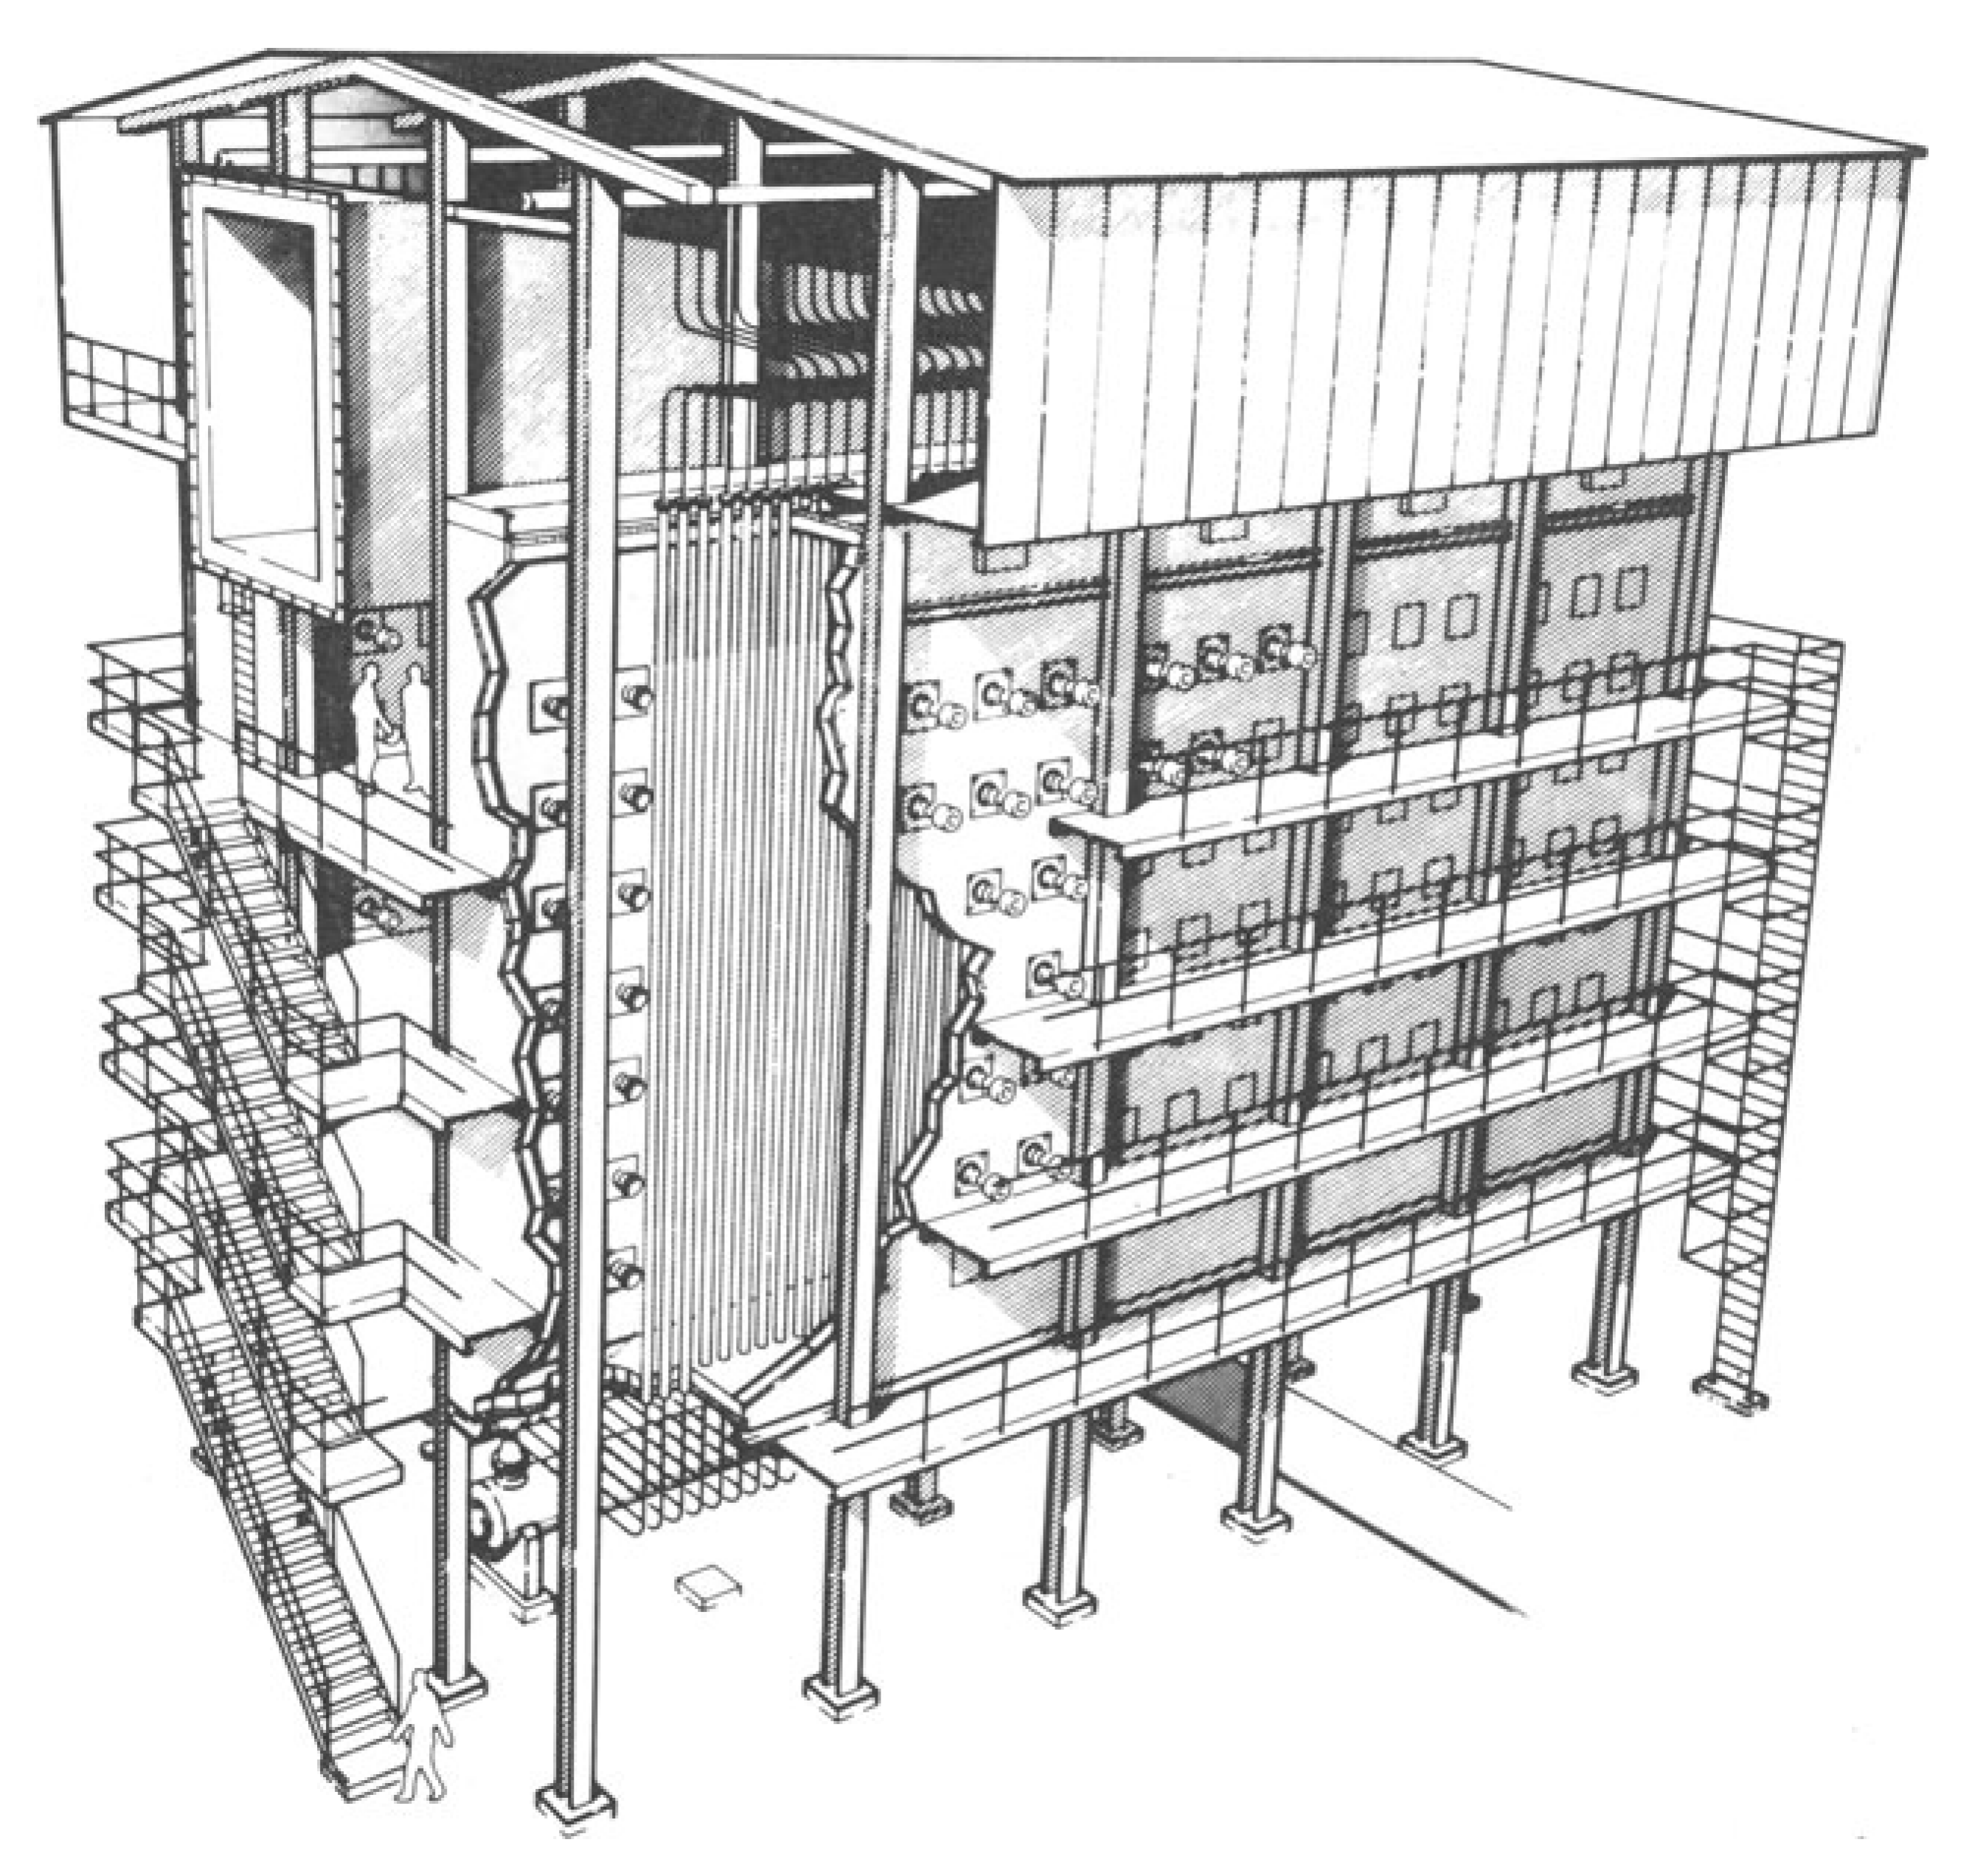
\includegraphics{figures/reformer-furnace}
\caption{Illustration of a typical reformer furnace. The reformer catalyst tubes are arranged vertically, with side-mounted burners on both walls. The pre-heated feedstock gas mixture enters the tubes from the top and the product gas is collected in an outlet manifold at the bottom of the furnace.  From \citet[Fig.~9]{rostrup-nielsen_catalytic_1984}.}
\label{fig:reformer-furnace}
\end{figure}

\begin{figure}[h]
\centering
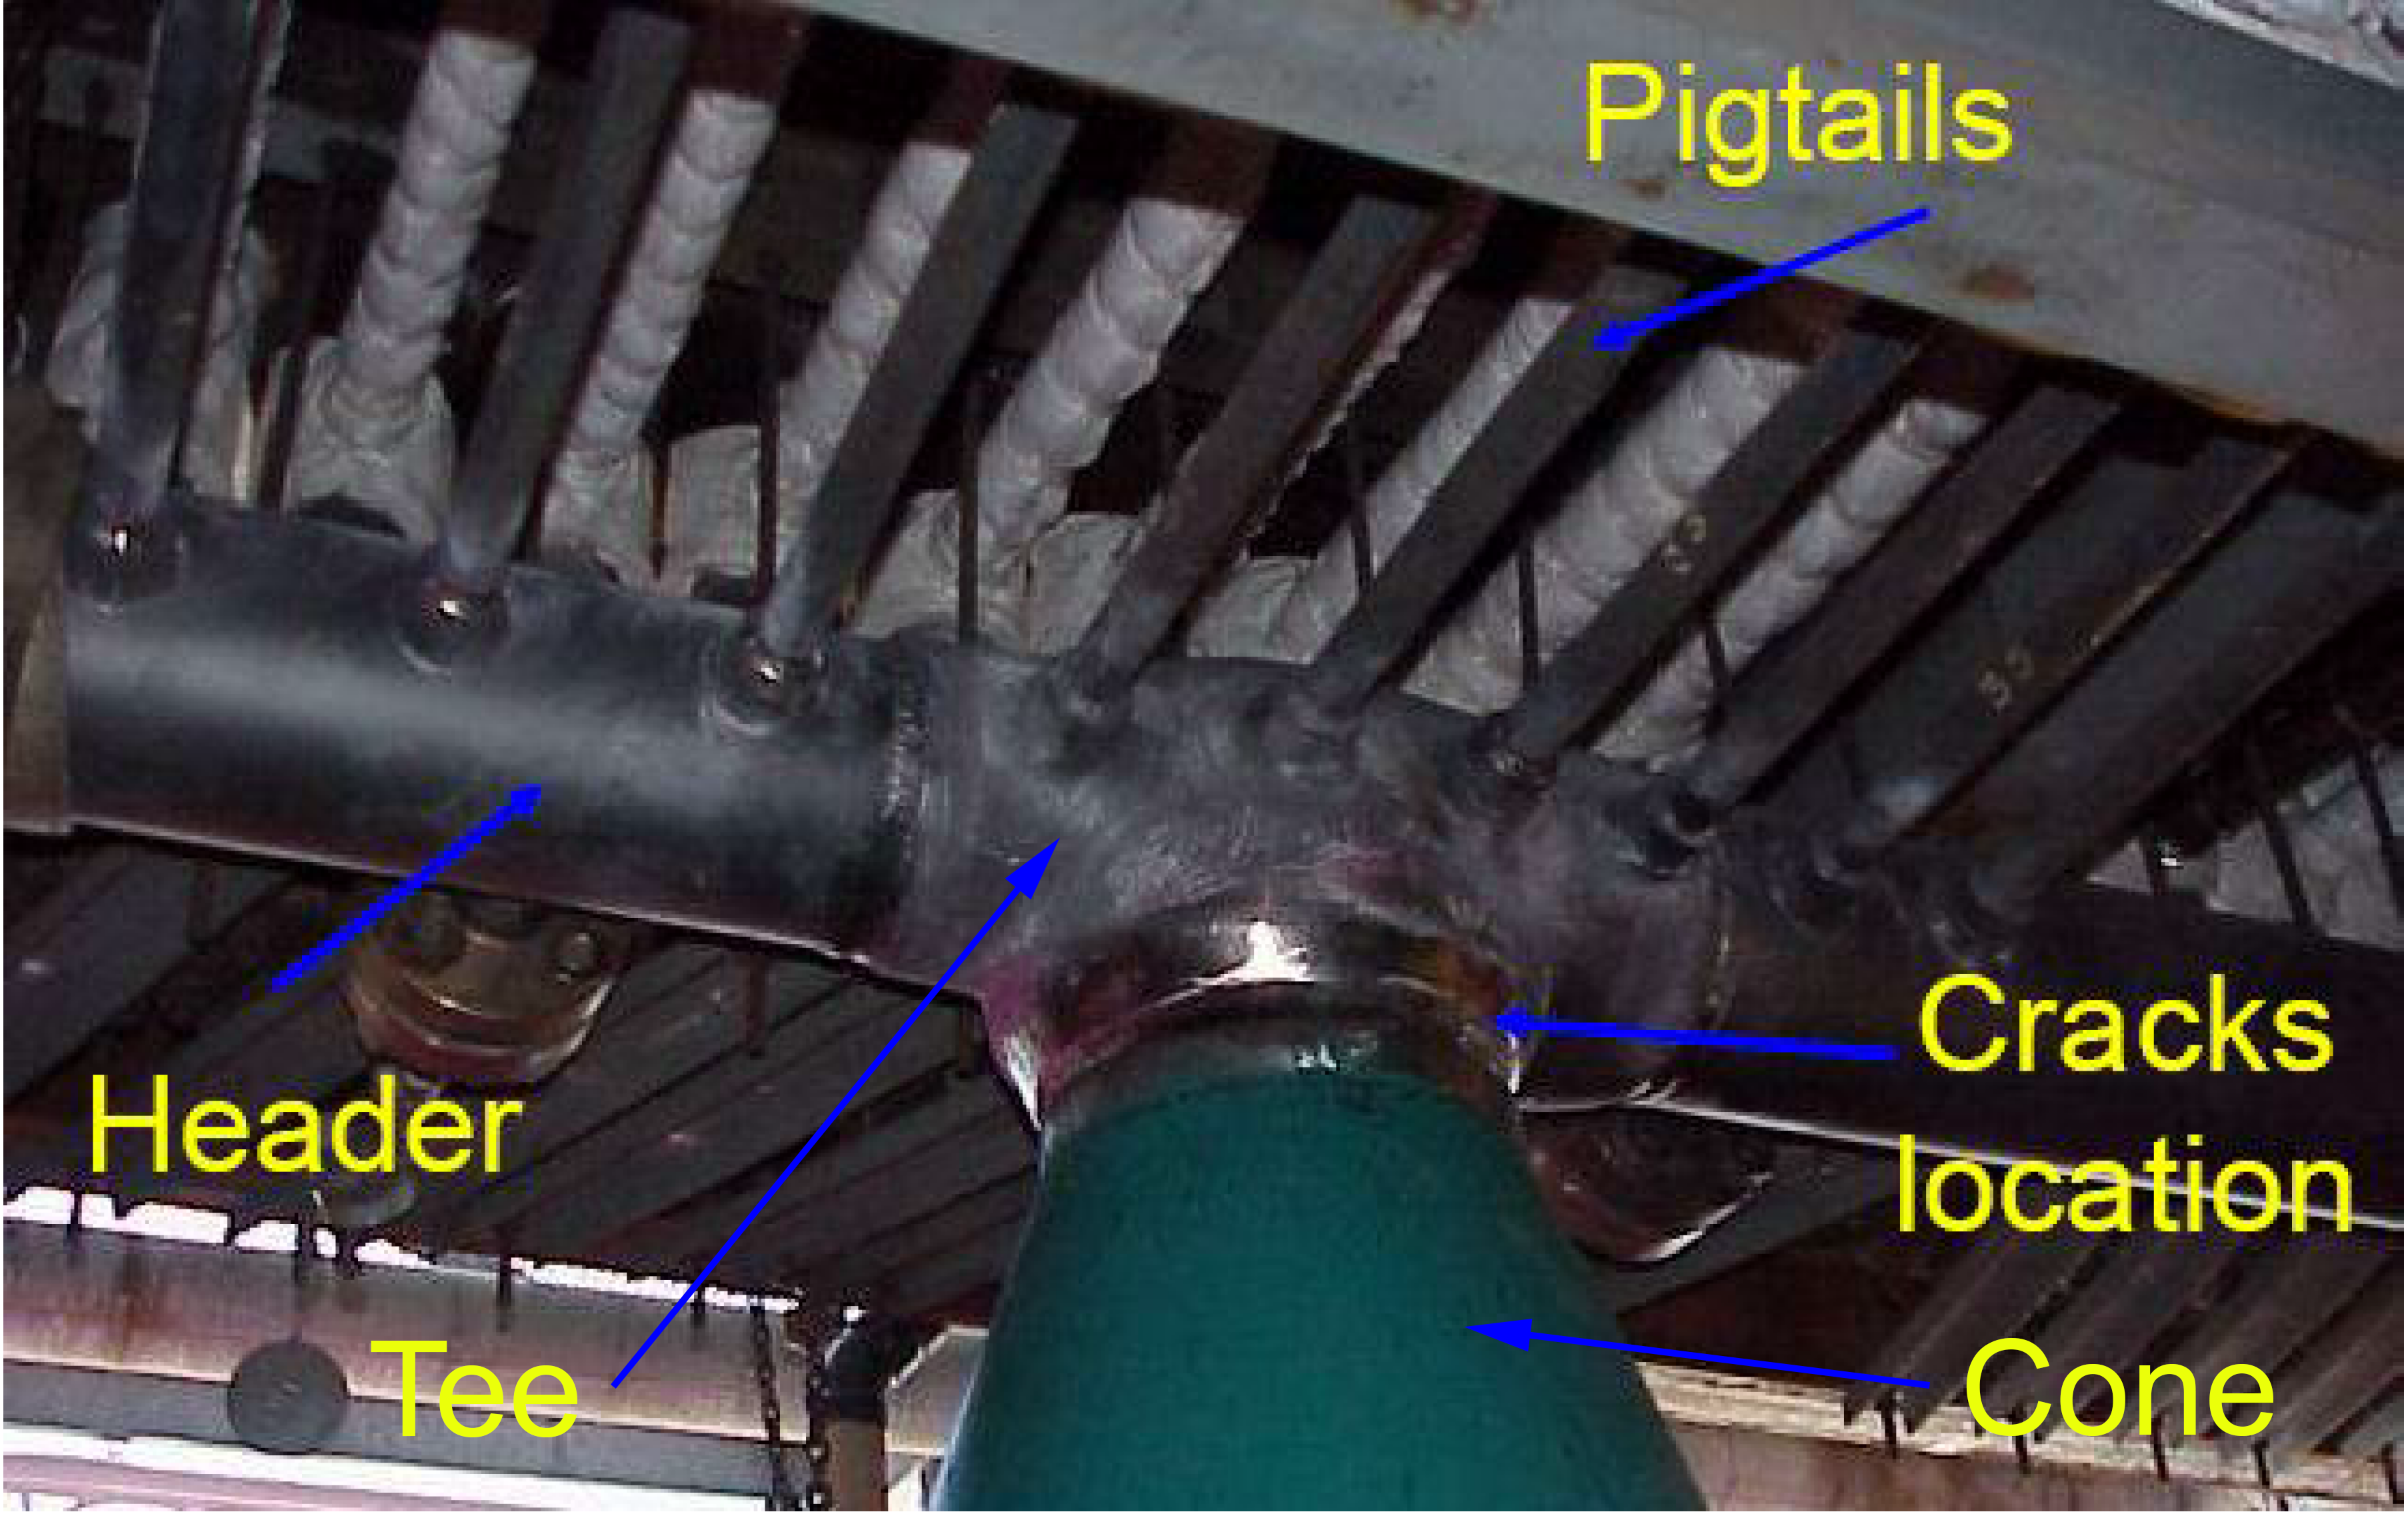
\includegraphics{figures/reformer-tee-cone}
\caption{Photograph of the outlet side of a reformer furnace, showing the outlet pigtails from the reformer catalyst tubes and the outlet header, tee, and cone which connect to the refractory-lined transfer system.  From \citet{penso_repair_2006}.}
\label{fig:reformer-tee-cone}
\end{figure}

Because high exit temperatures maximize the yield of hydrogen from the reformer \cite{haussinger_hydrogen_2000}, typical temperatures are in the range of 700--900C on the outlet side of the reformer furnace. Thus, the reformer tubes and outlet manifold require materials possessing excellent creep performance in addition to resistance to carburization and oxidation. The traditional choice for reformer tubes was centrifugally cast HK-40 (20Cr-25Ni) alloy \cite{rostrup-nielsen_catalytic_1984}, although this has been supplanted by newer alloys such as the HP-Modified alloys (25Cr-35Ni) due to higher creep strength \cite{schillmoller_hp-modified_1992}. For outlet manifold components, Alloy 800, HU-40 (19Cr-39Ni), and HK-40 have been used previously \cite{shibasaki_experience_1993}. The HU-40 and HK-40 alloys were implemented because they offered higher creep strength than Alloy 800, but they were discovered to have problems either with excessive thermal gradients (for HU-40), which was the same problem as originally experienced with Alloy 800, or with unacceptable loss of ductility after long-term service exposure (HK-40) \cite{shibasaki_experience_1993,collins_effect_1980}. To increase the ductilty after service exposure while maintaining high creep strength, a cast steel with the nominal composition of 20Cr-32Ni-1Nb was developed \cite{collins_effect_1980}. This alloy, which is specified as Grade CT15C in ASTM A351 \cite{astm_a351_2010}, has similar creep strength to HK-40 \cite{shibasaki_experience_1993} with improved ductility after service-exposure. 

Despite these improvements over traditional alloys, over the years industry has become aware \cite{api_942_2014} that the 20Cr-32Ni-1Nb alloy exhibits significant issues when it is subjected to repair welding after service exposure. These issues manifest primarily as cracking occurring in the base metal \gls{haz}, for example as reported by \citet{hoffman_weld_1998}. The cracking occurrences are not alleviated by changes to welding procedures, such as utilizing a more ductile filler metal, but rather are only prevented by high-temperature solution annealing (>2000\textdegree{}F) of the service-exposed material prior to welding. Thus the cracking issues are directly related to the microstructural changes which occur under service conditions (700--900C). The objective of the current work is to evaluate the weldability of service-exposed 20Cr-32Ni-1Nb material, utilizing a well-established test method for characterizing the weldability of steels (the Gleeble hot ductility test), and to relate the hot ductility results to observed microstructural characteristics.


% Due to high exit temperatures in the range of 700--900C on the outlet side of the reformer furnace, the reformer tubes and outlet manifold require materials possessing excellent creep performance. 


% Because the efficiency of the reforming reactions are linked to the exit temperature, materials with excellent creep performance are necessary for both the reformer tubes and outlet manifold to enable high operating temperatures to ensure high yield.


% Because the efficiency of the reforming reactions are dependent upon maintaining a high exit temperature, materials with excellent creep performance are necessary for both the reformer tubes and outlet manifold to enable high operating temperatures to ensure high yield.


% how does tube creep properties influence tube design?


% Because the reaction in 1 is endothermic while 2 and 3 are exothermic, the overall heat balance is negative under most process conditions and external heat must be supplied. Thus, steam reforming occurs in a reformer furnace having numerous reformer tubes which contain the catalyst material and through which the reactants are passed. 


